\documentclass[a4paper, 11pt]{article}

\usepackage[utf8]{inputenc}

\usepackage[T1]{fontenc}

\usepackage[french]{babel}

\usepackage{graphicx}

\usepackage[margin = 1in]{geometry}

\usepackage{fancyhdr}

\usepackage{float}

\usepackage{biblatex}

\usepackage{csquotes}

\addbibresource{references.bib}


\title{\Large LBIO1355 – Rapport de TP \\
\huge La co-évolution entre les Eulophidae et les Cassidinae}


\author{Gashi Vandenhove Elfie & Guyot Léopold & Hiernaux Stéphane}

\date{\today}
\begin{document}
\begin{titlepage}
   \begin{center}
       \vspace*{1cm}

        \LARGE
       \textbf{ LBIO1355 – Rapport de TP}

       \vspace{0.5cm}
       \Large
       La co-évolution entre les Eulophidae et les Cassidinae
            
       \vspace{1.5cm}
        \Large
       \textbf{Gashi Vandenhove Elfie\\ Guyot Léopold\\ Hiernaux Stéphane}

       \vfill
       \vspace{0.8cm}
     
       
\includegraphics[width=0.6\textwidth]{UCLouvain_Logo_Pos_CMJN.pdf}
            
      \large LBIO1355 – Rapport de TP\\
       Université catholique de Louvain-la-Neuve\\
       Belgique\\
       \today
            
   \end{center}
\end{titlepage}


\pagestyle{fancy}
\fancyhead{}\fancyfoot{}
\fancyhead[L]{
\includegraphics[width = 0.2\textwidth]{UCLouvain_Logo_Pos_CMJN.pdf}}
\fancyhead[R]{La co-évolution entre les Eulophidae et les Cassidinae}
\section{Introduction}
Nous savons tous que l’évolution est le mécanisme clé de la diversité des espèces. Au sein de l’évolution, la coévolution est un processus particulier lors duquel deux espèces évoluent en parallèle, influençant l’une et l’autre leur fitness. Dans ce rapport, nous allons étudier les arbres phylogénétiques de deux familles/sous-familles liées par une relation hôte-parasite afin de prouver leur coévolution. Celles-ci sont d’une part Eulophidae, une famille d’insectes hyménoptères parasitoïdes et plus grands représentants de la super-famille des Chalcidoidea, et d’autre part Cassidinae, une sous-famille d’insectes coléoptères de la famille des Chysomelidae. Ces Cassidinae sont souvent dépendants d’une plante hôte spécifique (Cuignet et al. 2007). Du fait de cette propension à toujours se localiser sur les mêmes familles de plantes, les membres de cette sous-famille sont des proies facilement trouvables pour les prédateurs et les parasites, faisant des Cassidinae la famille la plus parasitée au sein des Chrysomelidae. Cette pression sélective aurait donc mené à de nombreuses évolutions défensives à tous stades de développement chez cette famille (Olmstead 1994).
Le but de ce rapport est de prouver la coévolution entre nos deux familles en opposant les arbres phylogénétiques que nous obtiendrons en comparant des séquences d’ADN homologues. Selon la loi de Farenholz, la phylogénie des parasitoïdes et en miroir avec celle de leurs hôtes (Cuignet 2005). Nous allons donc vérifier si c’est bien le cas et à quel point ces arbres sont-ils l’image de l’autre une fois mis en vis-à-vis.


\section{Choix du marqueur pour les Eulophidae}

\subsection{Marqueur : 28S D2, ITS2 ou CytB ?} 

\subsection{Justification ?}

\section{Méthode de construction d'arbre Eulophidae (parasitoïdes)}

\textit{Soyez précis ! Méthode, modèle, … vous pouvez vous aider de captures d’écran. Pensez à justifier vos choix.}

\section{Méthode de construction d'arbre Cassidinae (hôtes)}

\emph{Soyez précis ! Méthode, modèle, … vous pouvez vous aider de captures d’écran. Pensez à justifier vos choix.}

\section{Arbre Eulophidae (parasitoïdes)}
\subsection{Format parenthétique} 


\subsection{Graphe :}

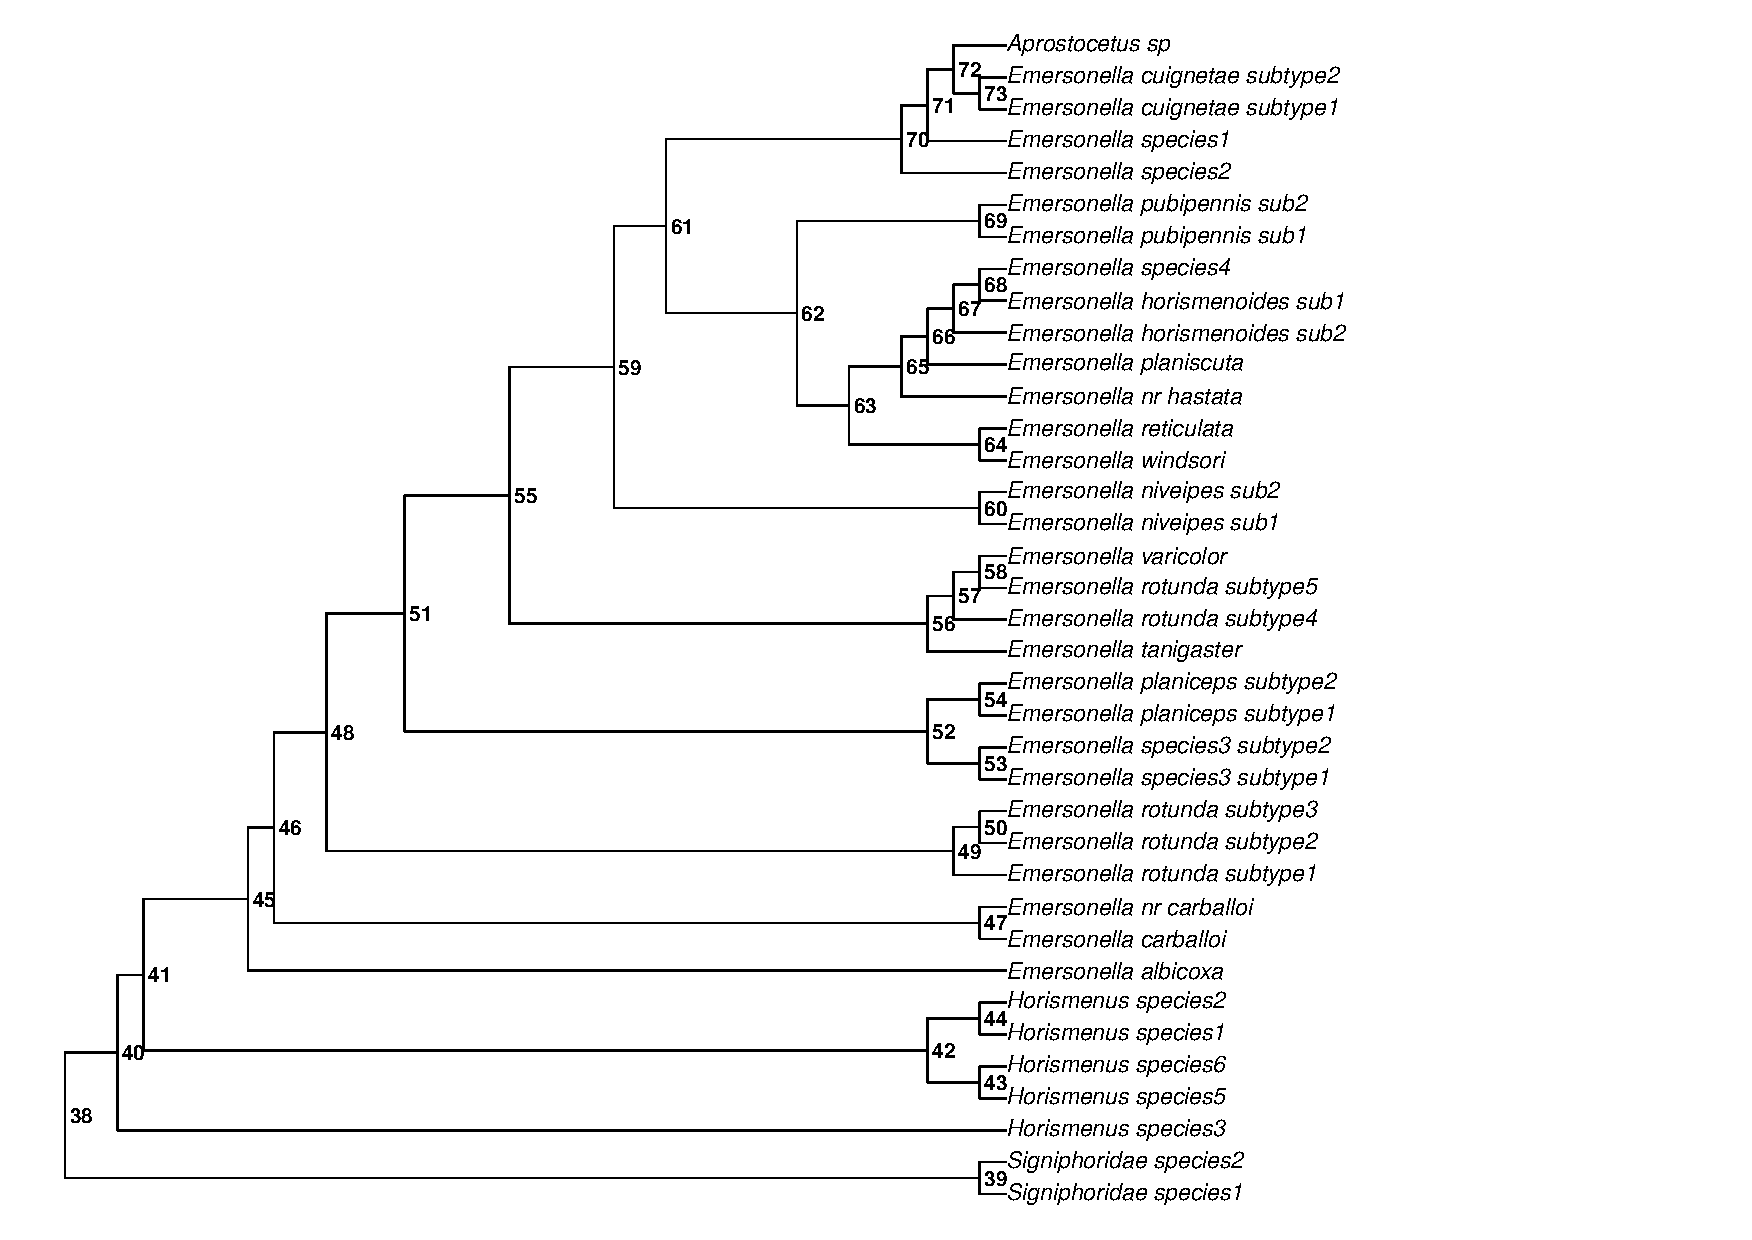
\includegraphics[width = 1\textwidth]{plot_Eulo_Cyt_b_PhyML_GTR_modified.pdf}
\subsection{Discussion}
\emph{Quelle fiabilité accordez-vous à votre arbre ? De quels regroupements êtes-vous sûrs ou les plus confiants ? Que proposeriez-vous pour améliorer votre résultat ?}

\emph{Discutez d’abord la topologie sans vous préoccuper des valeurs de bootstraps, puis en en tenant compte.}

\section{Arbre Cassidinae (hôtes)}
\subsection{Format parenthétique} 


\subsection{Graphe :}
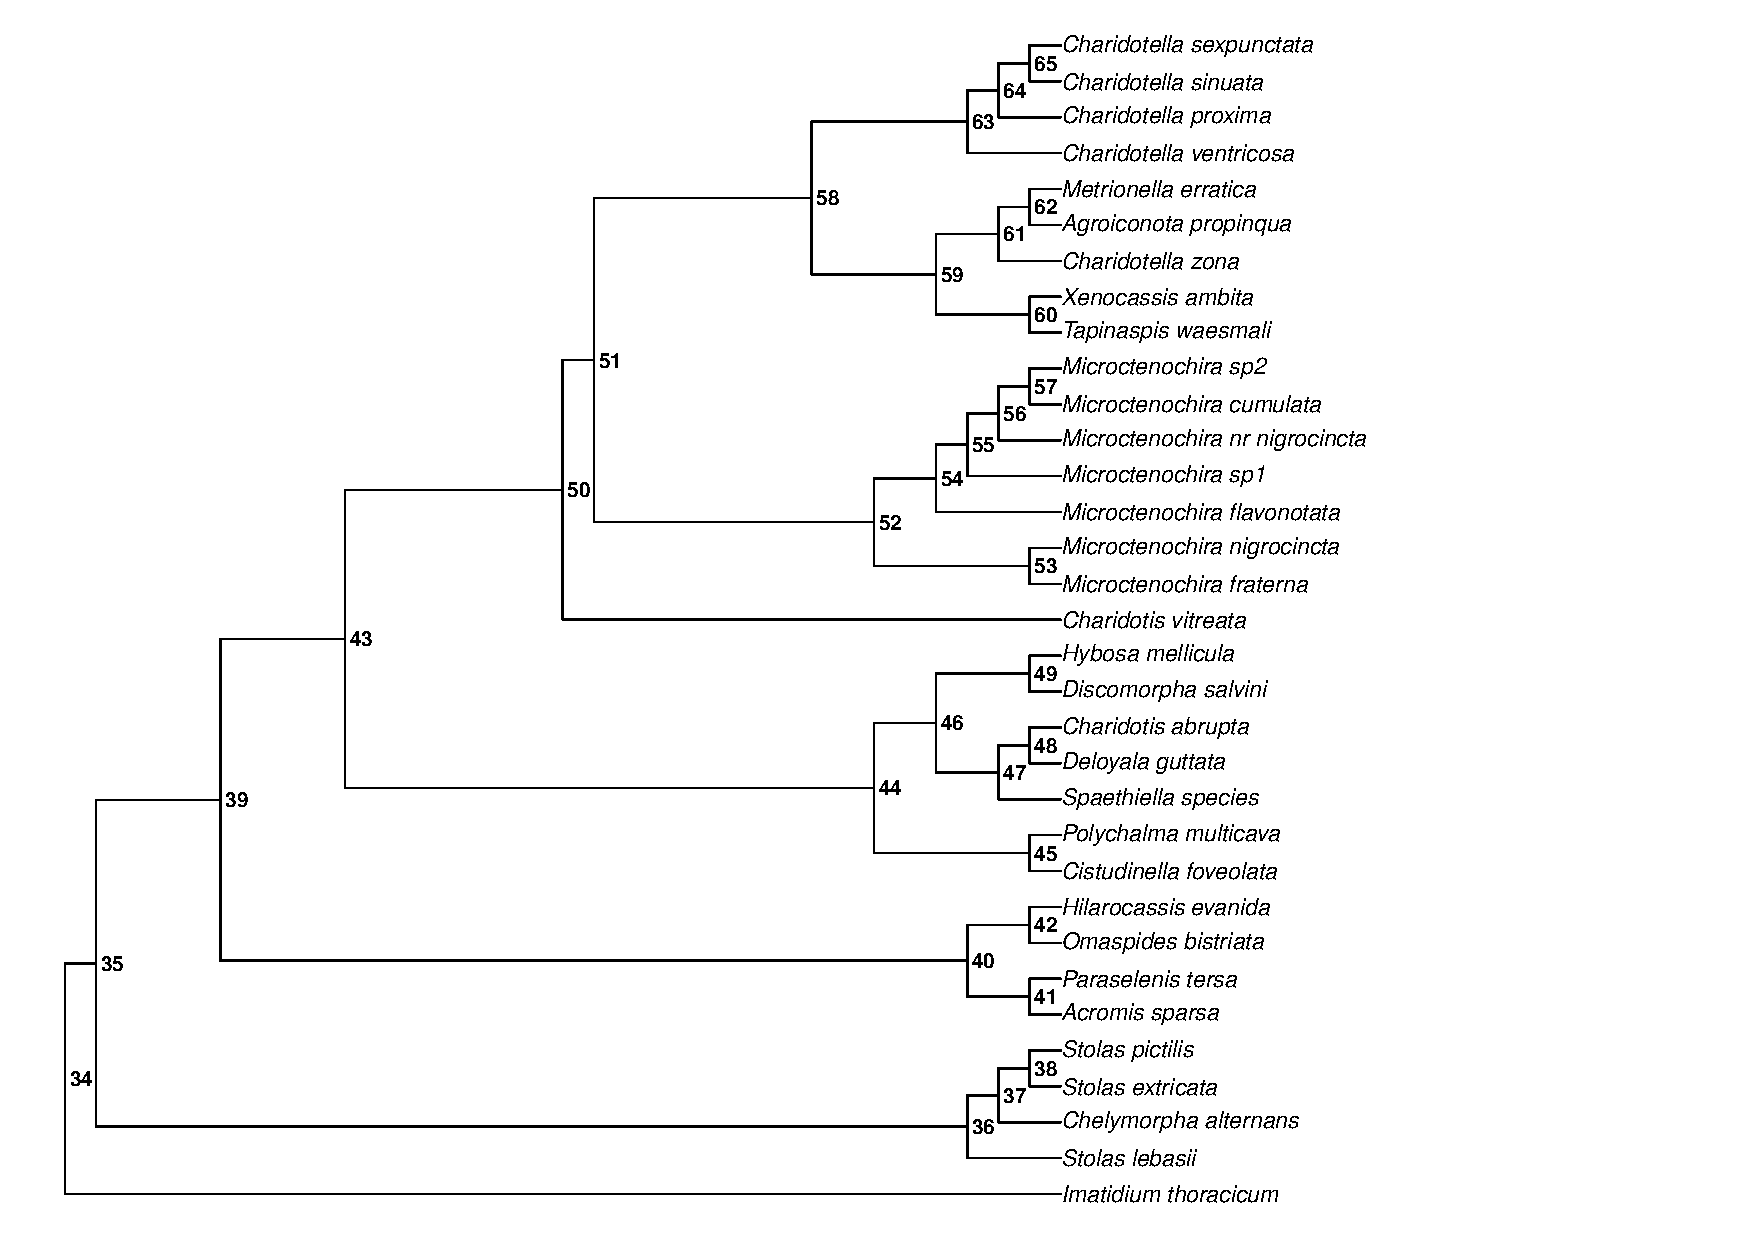
\includegraphics[width = 1\textwidth]{plot_Cassidinae_28S_D2_PhyML_GTR.pdf}
\subsection{Discussion}
\emph{Quelle fiabilité accordez-vous à votre arbre ? De quels regroupements êtes-vous sûrs ou les plus confiants ? Que proposeriez-vous pour améliorer votre résultat ?}
\emph{
Discutez d’abord la topologie sans vous préoccuper des valeurs de bootstraps, puis en en tenant compte.}
On peut tout d’abord observer sur l’arbre des \emph{Cassidinae} (citer fig.) un outgroup constitué d’\emph{Imatidium thoracicum}.\\
Concernant le reste de l’arbre, les différentes espèces d’un même genre sont presque toutes regroupées sous un nœud unique ce qui peut être un bon indicateur de la solidité (notamment au sein des genres \emph{Microctenochira}, \emph{Charidotella}et \emph{Stolas}). Toutefois, on observe aussi des espèces isolées des autres espèces d’un même genre, c’est le cas de \emph{Charidotella zona}, des 2 espèces du genre \emph{Charidotis} ainsi que \emph{Stolas lebasii}. Le fait que la classification de ces espèces se soient faite sur base de caractères morphologiques et le manque d’analyse génomique au sein de la sous-famille des \emph{Cassidinae} pourraient expliquer la paraphylie rencontrée.\\
Un autre facteur ayant pu jouer sont les valeurs de bootstraps. Il est possible d’en observer quelques-unes un peu plus faibles, notamment au niveau des genres paraphylétiques. Toutefois, on retrouve plusieurs valeurs supérieures à 80 ce qui peut appuyer la solidité de notre arbre. Bien que faire plus de réplicas de notre arbre aurait permis d’avoir des résultats plus fiables. De plus, on observer à certains nœuds trois embranchements.\\ 
Finalement, il aurait été intéressant de comparer des arbres faits avec différentes méthodes mais les autres arbres obtenus avaient des valeurs de bootstraps trop faibles et les analyser n’aurait pas été pertinent.


\section{Coévolution}

\subsection{Graphe (les deux arbres, et les liens entre eux)}
\emph{Soyez clairs / illustratifs. N’hésitez pas à remettre en forme via R, Powerpoint…}

\subsection{Discussion}
\emph{Y a-t-il selon vous coévolution ? Dans quelle mesure ?}
\section{Conclusion}
\emph{Soyez clairs, concis, synthétiques, cohérents, mais aussi exhaustifs ! La conclusion, c’est la fin de l’histoire, c’est la finalisation du travail. En tant que telle, elle se doit d’en rappeler tous les points importants, de les représenter de manière cohérente, et de montrer ce qu’il a apporté (ce que nous savons en plus et que nous ne savions pas au début). Éventuellement, cette conclusion peut également comprendre une critique constructive et des perspectives.}

\printbibliography

\section{Annexes (.fasta)}

\end{document}
